\section{Prototype of personalized bio-mechanical knee}

The work done in this section was in collaboration with Alex Tacescu. I led and managed the focus of the project and came up with the idea. I was also involved with running the mocap experiments and the mechanical design. Another knee design was examined that focused on matching the knee motion profile to a human knee. Exoskeletons discussed in \autoref{sec:ExoBack} mostly use pin-type joints in their knee joints; this is in contrast to how the actual kinematics work in a human knew, which has a variable center of rotation \cite{morrison1970mechanics} \cite{koo2008knee}.

Several recent designs have focused more on accounting for knee motion. Choi \textit{et. al} used multiple rolling cams to adapt to the changing center of rotation \cite{choi2017development}. This design fits a person's knee motion; it did not use modeling of the knee's tibiofemoral motion to design the cams. Additionally, the design is complicated and not easily reproducible. In another design Choi \textit{et. al} used multiple rollers and pulleys powered by electric linear actuators. However, rotary electric motors with rotary gearboxes can often achieve higher performance than electric linear actuators powered by rotary DC motors. Another knee design was presented in \cite{wang2018comfort}; this design prioritized the comfort of the user and the alignment of the knee joint. This design also uses pulleys and cables to model the knee motion. \cite{AdaptiveKneeJoint} presents a cam knee design that uses a model of the knee motion. This design is a significant improvement over previous designs that merely compensate for the motion. However, as the other designs discussed, they use linear actuators.  These designs do well at either mimicking or compensating for the knee motion; however, they are mechanically cumbersome to manufacture; they did not show mimicking of the center of rotation's theoretical movement and/or use a linear actuator to replicate rotary motion. In addition, the design does not allow for the knee to be customized and therefore cannot meet the specific motion of the patient. Thus, we propose a knee design that is readily configured to match a particular patient's knee joint motion, is designed for easy manufacturing, and allows the use of readily available rotary actuators and brake mechanisms.

The variable center of rotation was found using previous work by Iwaki \textit{et. al} that used Magnetic Resonance Imaging (MRI) scans to determine and predict the knee's trajectory \cite{MRIKneeShape_Loaded, MRIKneeShape_Unloaded}. These studies used cadavers and actual patients to measure the motion of the knee in both loaded and unloaded scenarios. This MRI data was used in \cite{KinDynKneeJoint} to build a mathematical model of knee motion that considers both the flexion and extension degrees of freedom. They used ellipse to model the contact between the femur and tibia bones. Their work leads to the formulation of \autoref{eq:KneeExtensionFlexionNumeric}. This equation relates the rotation of the knee to the translation of the tibia. This motion and its derivative are shown in \autoref{fig:FlexExtRelationship}. This study was limited since it was based on the anthropomorphic parameters of a single person. These coefficients will vary slightly from person to person and can be found using MRIs or motion capture. 


\begin{equation}
    r(\theta) mm = 1.078\theta^4 - 11.184\theta^3 + 26.524\theta^2 - 0.825\theta + 263.59
    \label{eq:KneeExtensionFlexionNumeric}
\end{equation}

\begin{figure}[ht!]
    \centering
    \includegraphics[scale=0.9]{images/mech_design/FlexionCurve.png}
    \caption{Knee Flexion Curve}{Graphical representation of \autoref{eq:KneeExtensionFlexionNumeric} demonstrating the relationship between flexion and extension in a knee as measured by \cite{KinDynKneeJoint}. \(r(m)\) is the extension distance between the center of the knee and the center of mass of the lower leg. $0^\circ$ represents a perfectly extended knee joint.}
    \label{fig:FlexExtRelationship}
\end{figure} 

A cam-type mechanism with a brushless DC motor was designed to follow the desired path. The guide was generated using \autoref{eq:KneeExtensionFlexionNumeric}. This guide enforces variable center of rotation and motion of the tibia. \autoref{fig:ExplodedViewLabeled} shows an exploded view of the knee mechanism. 



\begin{figure}
    \begin{subfigure}{\textwidth}
        \centering
        \captionsetup{justification=centering}
        \includegraphics[scale=0.2]{images/mech_design/ExoKneeExplodedView.png}
        \caption{Bio Knee joint design exploded view}{Knee joint design exploded view}
        \label{fig:ExplodedViewLabeled}
    \end{subfigure}
    \begin{subfigure}{\textwidth}
        \centering
         \includegraphics[scale=0.2]{images/mech_design/KneeJointAssyCrossSection.png}
          \captionsetup{justification=centering}
        \caption{Cross section of Bio knee}{A cross section of the knee joint with the potentiometer embedded in the design. The wires are routed along the wire channel to avoid interference with the inner arm and plastic slides}
        \label{fig:CrossSectionPot}
    \end{subfigure}    
    \caption{Exploded View of bio-knee mechanism}
    \label{fig:bioknee}
\end{figure}

The motor and gearbox need to provide sufficient torque and power to drive the knee of a $100kg$ patient through gait motion. This mass is larger than the average mass of the North American paraplegic, which is $68.8kg$, so assuming a larger mass allows for the motor to have a safety factor. Additionally, it is assumed that the dynamic loads are assumed to be negligible during the slow-motion collision with the ground. It equates to approximately $65W$ of power and $25Nm$ of torque at \(15^\circ/sec\). The knee is powered by a $90W$ brushless Maxon motor used with a nominal torque of $0.56Nm$ at roughly $2500rpm$.  The motor is combined with a Harmonic gearbox with a $100:1$ reduction. \autoref{table:MotorGearboxSpecs} shows the gearbox and motor specifications and the joint's mechanical properties. The calculations assumed an efficiency of \(90\%\) as per the manufacturer documentation. The designed knee joint can mechanically output $81W$ and $50.4Nm$ at $15^\circ/sec$.  

\begin{table}
    \centering
    \begin{tabular}{||c|c|c||}
        \hline
        Input (Motor) Power & \(P_{input}\) & \(90 Watts\) \\
        \hline
        Input (Motor) Torque @ Nominal & \(\tau_{input}\) & \(0.560 Nm\) \\
        \hline
        Input (Motor) Speed @ Nominal & \(\omega_{input}\) & \(2510 rpm\) \\
        \hline
        Input (Motor) Stall Torque & \(\tau_{in\_stall}\) & \(7.480 Nm\) \\
        \hline \hline
        Gearbox Ratio & \(\frac{n_1}{n_2}\) & \(100:1\) \\
        \hline \hline
        Output Power & \(P_{output}\) & \(81 Watts\) \\
        \hline
        Output Torque @ Nominal & \(\tau_{input}\) & \(50.4 Nm\) \\
        \hline
        Output Speed @ Nominal & \(\omega_{input}\) & \(15^\circ/sec\) \\
        \hline
        Output Stall Torque & \(\tau_{out\_stall}\) & \(673.2 Nm\) \\
        \hline
    \end{tabular}
    \caption{Bio Knee parameters}{Motor/gearbox specifications and output power specifications of the proposed joint.}
    \label{table:MotorGearboxSpecs}
\end{table}

The design was validated using a motion capture system and SolidWorks motion analysis \footnote{https://www.solidworks.com/category/simulation-solutions}. The markers on the knee were aligned on the shank and thigh segments of the knee and rotated through the desired motion as shown in \autoref{fig:KneeJointTestSetup}; this allowed us to compare the theoretical trajectory to the actual trajectory, and for the measurement and comparison of manufacturing tolerance. \autoref{fig:KneeJointTestResults} shows the results of the study. There are some slight deviations of the actual motion compared to the desired motion; this deviation is caused by hysteresis in the system. However, these movements are very slight on a scale of less than $1mm$, which is assumed to be negligible.   



\begin{figure}[ht!]
    \centering
    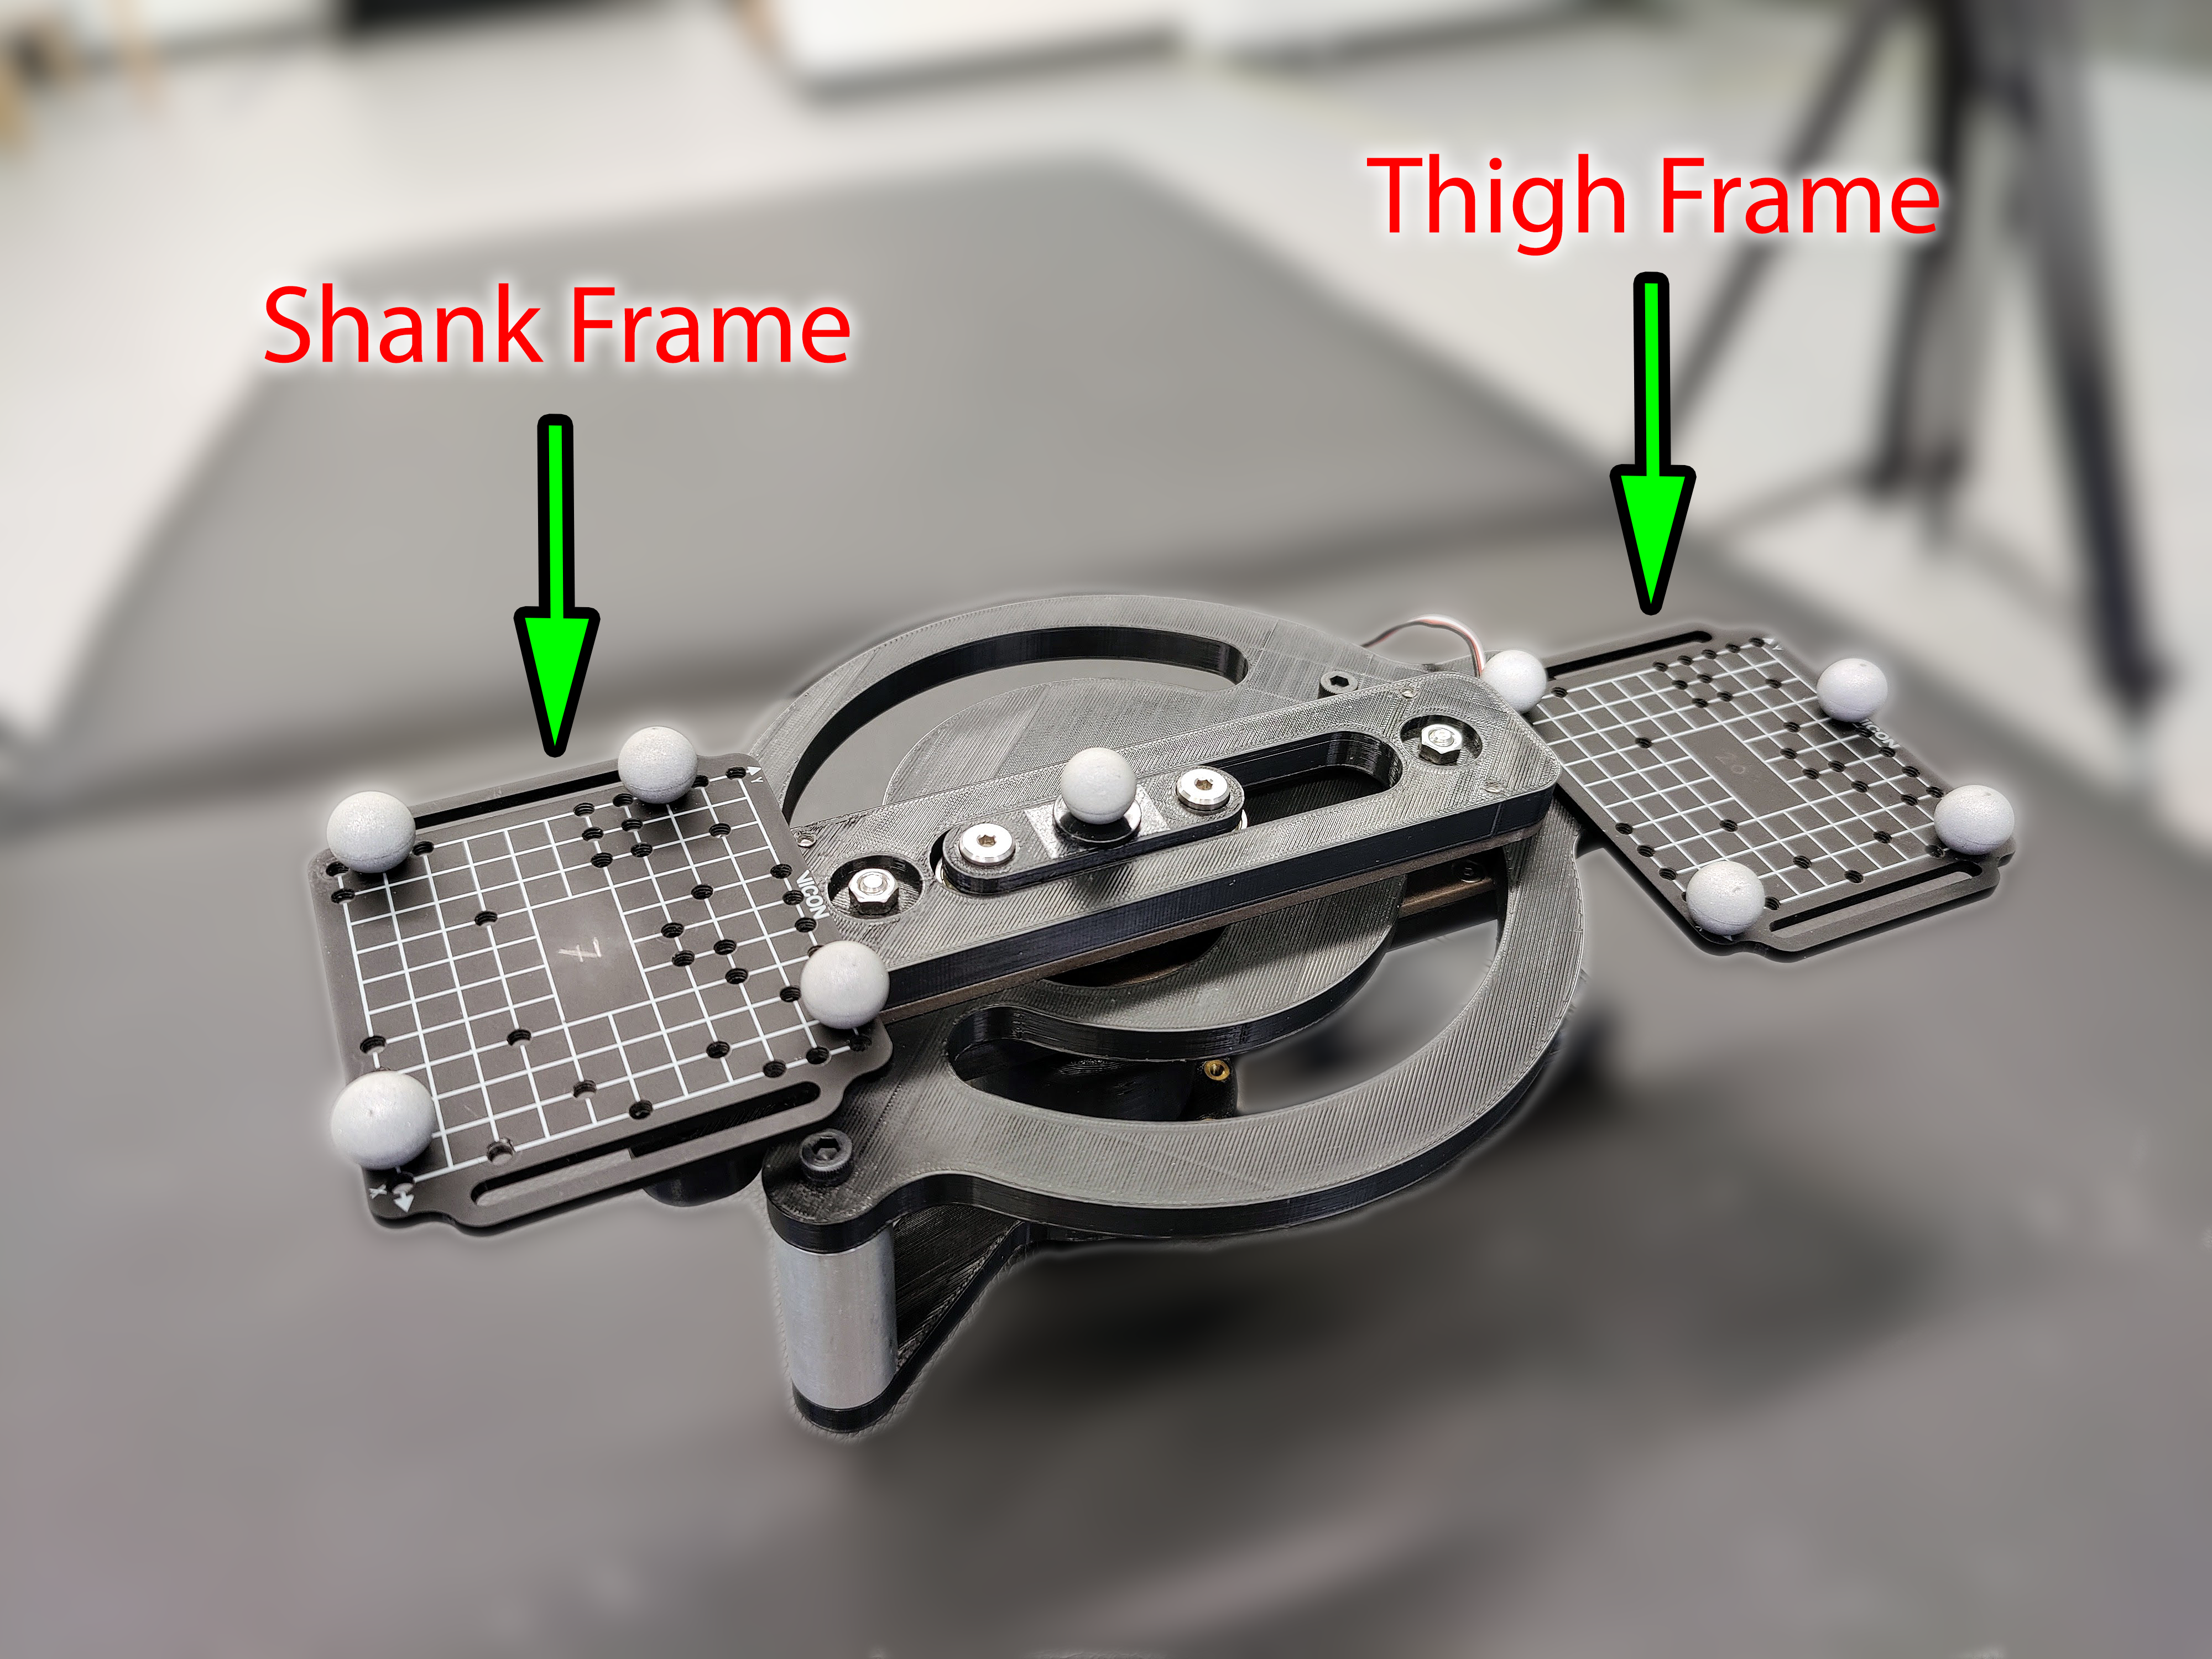
\includegraphics[scale=0.07]{images/mech_design/KneeTrajTest_edit.png}
    \caption{Knee with mocap markers}{Knee joint setup with motion capture dots}
    \label{fig:KneeJointTestSetup}
\end{figure}

\begin{figure}[ht!]
    \centering
    \includegraphics[scale=0.75]{images/mech_design/FlexionExtensionKneeJoint.png}
    \caption{Comparison of variable center of rotation}{Graph showing knee joint flexion vs linear extension of the radius of curvature for the goal trajectory (see \autoref{eq:KneeExtensionFlexionNumeric}) and the experimental results from the Motion Capture Study}
    \label{fig:KneeJointTestResults}
\end{figure}

This knee design is easily manufactured; the common parts are made from off-the-shelf parts. The only customizable component is the guide plate, 3D printed on a standard 3D printer. The path can be fitted to the individual's anthropomorphic parameters, 3D printed without understanding advanced manufacturing methods of techniques. 